\documentclass{article}

\usepackage[utf8]{inputenc}
\usepackage[T1]{fontenc}

\usepackage[yyyymmdd, hhmmss]{datetime}
\usepackage{graphicx}
\usepackage{float}
\usepackage{subcaption}

\usepackage{minted}
\usepackage[os=win]{menukeys}
\usepackage{tikz}

\usepackage[english]{babel}
\usepackage{geometry}

\usepackage{adjustbox}
\usepackage{multirow}
\usepackage{hyperref}
\usepackage{titlesec}

\geometry{
	a4paper,
	left=25mm,
	right=25mm,
	top=25mm,
	bottom=25mm,
}

\hypersetup{
	colorlinks=true,
	linkcolor=blue,
	urlcolor=blue,
}

\setcounter{secnumdepth}{4}
\renewcommand{\theparagraph}{\thesubsubsection.\alph{paragraph}}

\addto\captionsenglish{\renewcommand{\tablename}{Tabel}}
\addto\captionsenglish{\renewcommand{\figurename}{Gambar}}

\begin{document}
	\begin{titlepage}
		\centering

		{
			\LARGE
			\bf
			Uji Respon Headphone Menggunakan Ear Simulator
		}

		\bigskip

		{
			\large
			\bf
			Tim Penelitian Audiometer Portable
		}

		\vfill
	\end{titlepage}

	\newpage
	% \section{Pendahuluan}


	\section{Tujuan Pengujian}
	Pengujian resppon headphone bertujuan untuk memperoleh informasi berupa:
	\begin{itemize}
		\item Karakteristik respon dari headphone, meliputi: frequency response, harmonic distortion,
		\item Sound pressure level (SPL) dari luaran tone portable audiometer
	\end{itemize}

	\section{Metode Pengujian}
	\subsection{Alat dan Perangkat Pendukung}
	Pengujian ini memerlukan peralatan dan perangkat pendukung sebagai berikut:
	\begin{itemize}
		\item \textbf{Ear simulator}. Pada pengujian ini digunakan dua jenis Ear simulator, yaitu:
		\begin{enumerate}
			\item miniDSP EARS (\href{https://www.minidsp.com/images/documents/Product%20Brief-EARS.pdf}{detail produk})
			\begin{figure}[H]
				\centering
				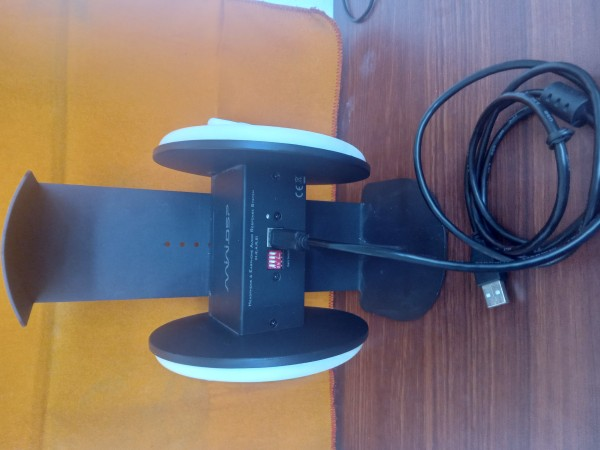
\includegraphics[width=200pt,angle=-90]{images/unit/ears}
				\caption{MiniDSP EARS}
			\end{figure}

			\item Free Space Pro II Binaural Microphone (\href{https://3diosound.com/products/free-space-pro-binaural-microphone}{detail produk})

			\begin{figure}[H]
				\centering
				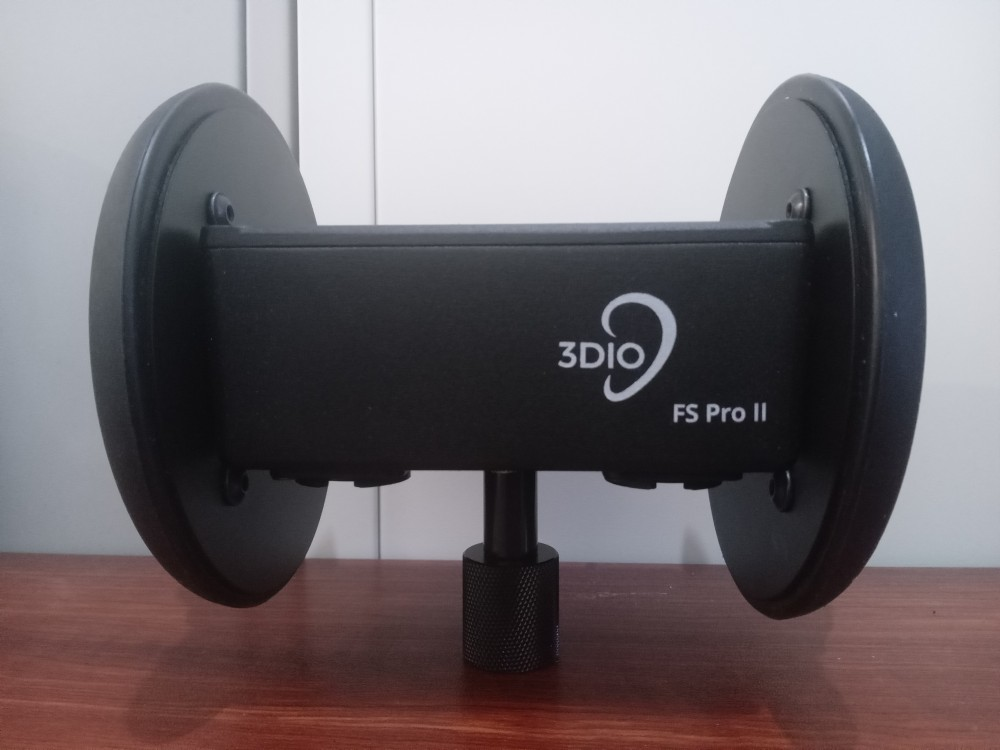
\includegraphics[width=200pt,angle=0]{images/fspro/fspro}
				\caption{Free Space Pro II}
			\end{figure}

			\newpage
			\item Presonus AudioBox USB96 (\href{https://www.presonus.com/en/interfaces/complete-recording-solutions/2777700101.html}{detail produk})

			\begin{figure}[H]
				\centering
				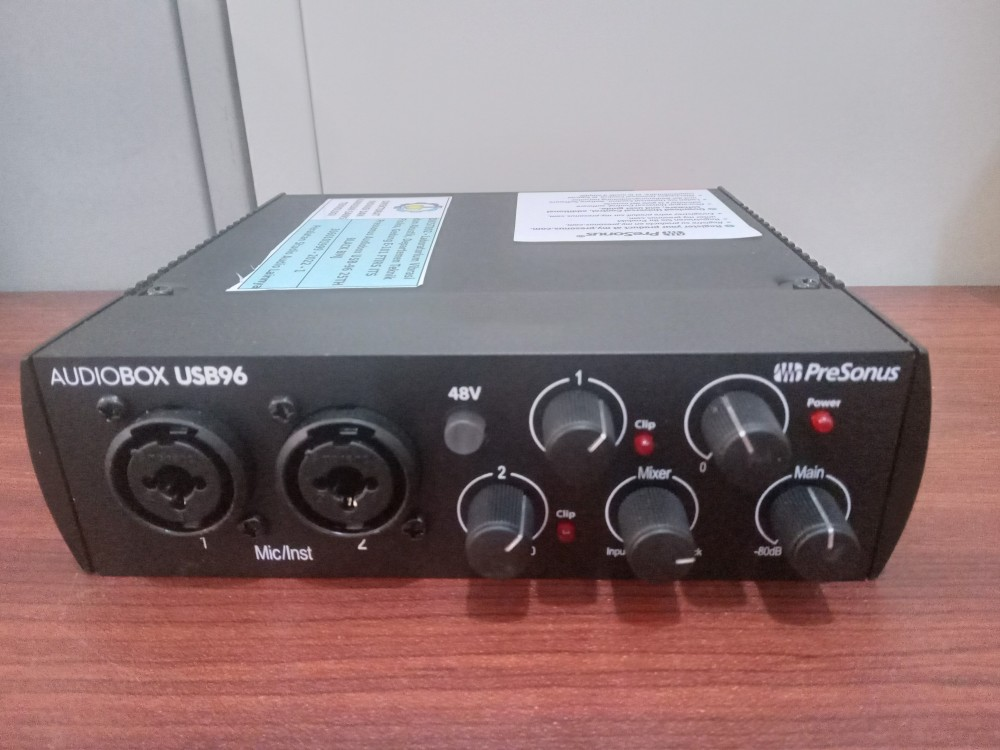
\includegraphics[width=180pt,angle=0]{images/fspro/presonus}
				\caption{USB96}
			\end{figure}

		\end{enumerate}

		\item \textbf{Headphone} yang akan diuji, yaitu:
		\begin{enumerate}
			\item JBL Tune 500 Wire On-Ear Headphone
			(\href{https://id.jbl.com/over-ear-headphones/JBL+TUNE500.html}{detail produk})
			\begin{figure}[H]
				\centering
				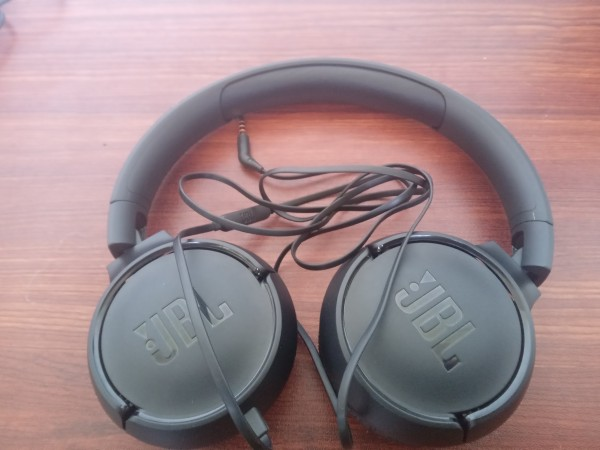
\includegraphics[width=180pt]{images/unit/jbl}
				\caption{Wired Headphone}
			\end{figure}

			\item Bose Frames Tempo Open-Ear Headphone
			(\href{https://www.bose.com/en_us/products/frames/bose-frames-tempo.html#v=bose_frames_tempo_black_us}{detail produk})
			\item IMOO Open-Ear Headphone
			(\href{https://imoostore.com/pages/imoo-ear-care-headset}{detail produk})
		\end{enumerate}

		\item Perangkat {\bf Audiometer Portabel}

		\begin{figure}[H]
			\centering
			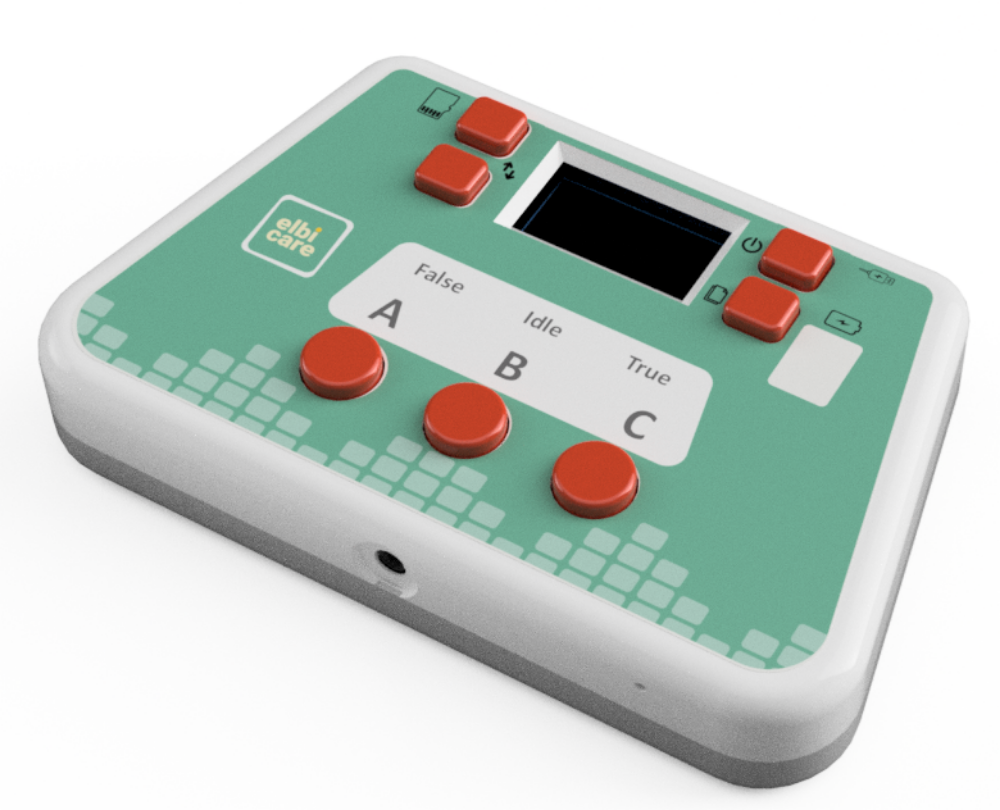
\includegraphics[width=180pt,angle=0]{images/elbicare}
			\caption{Elbicare Audiometri}
		\end{figure}

		\item Software \textbf{Room Equalization Wizard (REW)} (unduh \href{https://www.roomeqwizard.com/}{disini})
	\end{itemize}

	\newpage
	\subsection{Prosedur Pengujian}
	\subsubsection{Pengujian menggunakan miniDSP EARS}
	\paragraph{Pengukuran Karateristik Respon Headphone}
	\subparagraph{Setup dan Pengaturan Perangkat}
	\label{setup}
	\begin{enumerate}
		\item Atur nilai gain pada gain switch di panel depan miniDSP EARS (Gambar \ref{fig:front-panel}) mengikuti acuan pada Tabel \ref{table:gain}. Pada pengujiani ini digunakan nilai gain sebesar 18 dB.

		\begin{table}[H]
			\centering
			\caption{Pengaturan Gain pada MiniDSP EARS \label{table:gain}}
			\begin{tabular}{| p{0.1\textwidth} | p{0.1\textwidth} | p{0.1\textwidth} | p{0.1\textwidth} |}
				\hline
				Switch 1 & Switch 2 & Switch 3 & Gain (dB) \\ \hline\hline
				Down & Down & Up & 0 \\ \hline
				Down & Up & Down & 6 \\ \hline
				Down & Up & Up & 12 \\ \hline
				Up & Down & Down & 18 \\ \hline
				Up & Down & Up & 24 \\ \hline
				Up & Up & Down & 30 \\ \hline
				Up & Up & Up & 36 \\ \hline
			\end{tabular}
		\end{table}

		\begin{figure}[H]
			\centering
			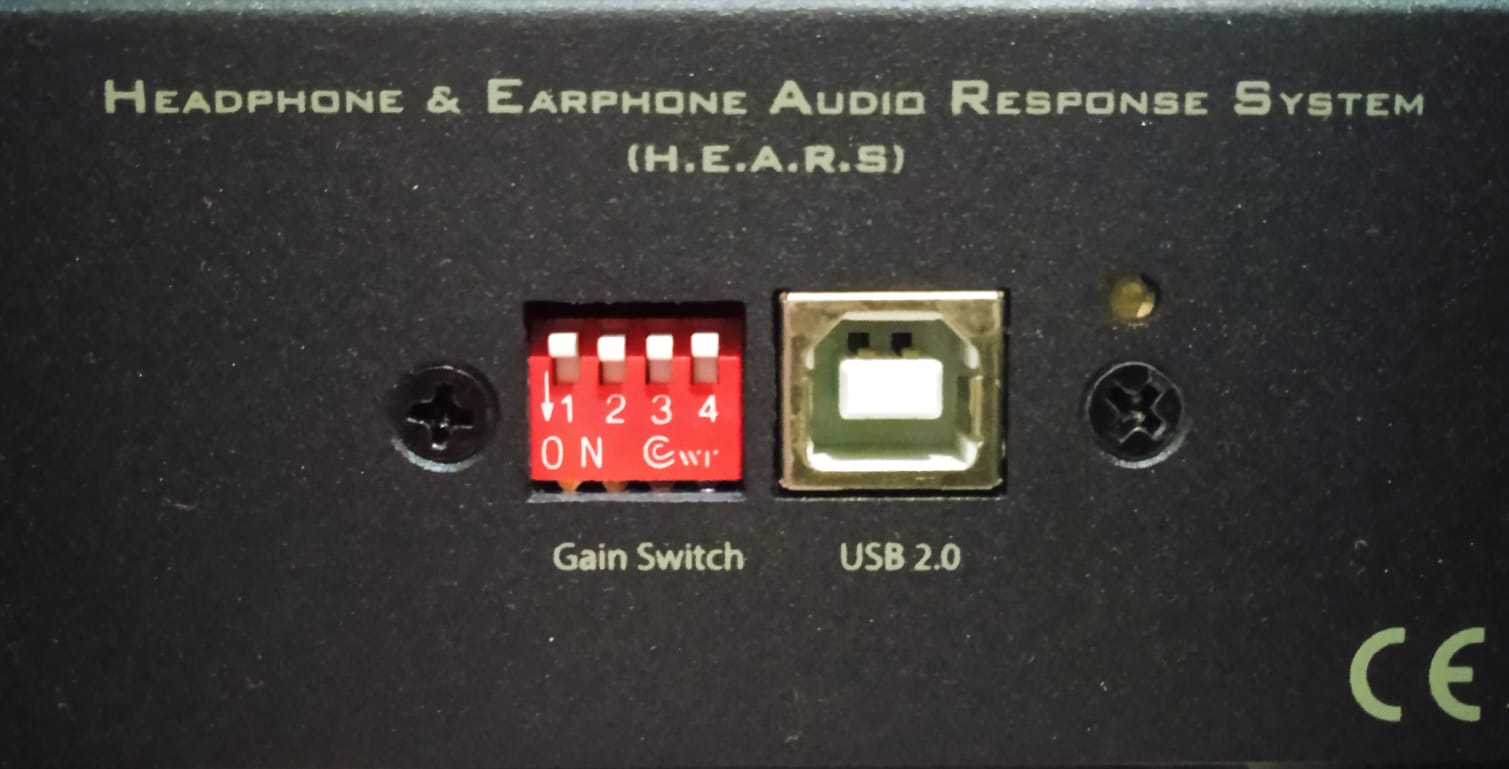
\includegraphics[width=0.5\textwidth]{images/front-panel}
			\caption{Tampilan panel depan miniDSP EARS}
			\label{fig:front-panel}
		\end{figure}

		\item Hubungkan miniDSP EARS ke laptop menggunakan sambungan kabel USB (Gambar \ref{fig:plug-in}) yang tersedia.

		\begin{figure}[H]
			\centering
			\begin{subfigure}[]{.45\textwidth}
				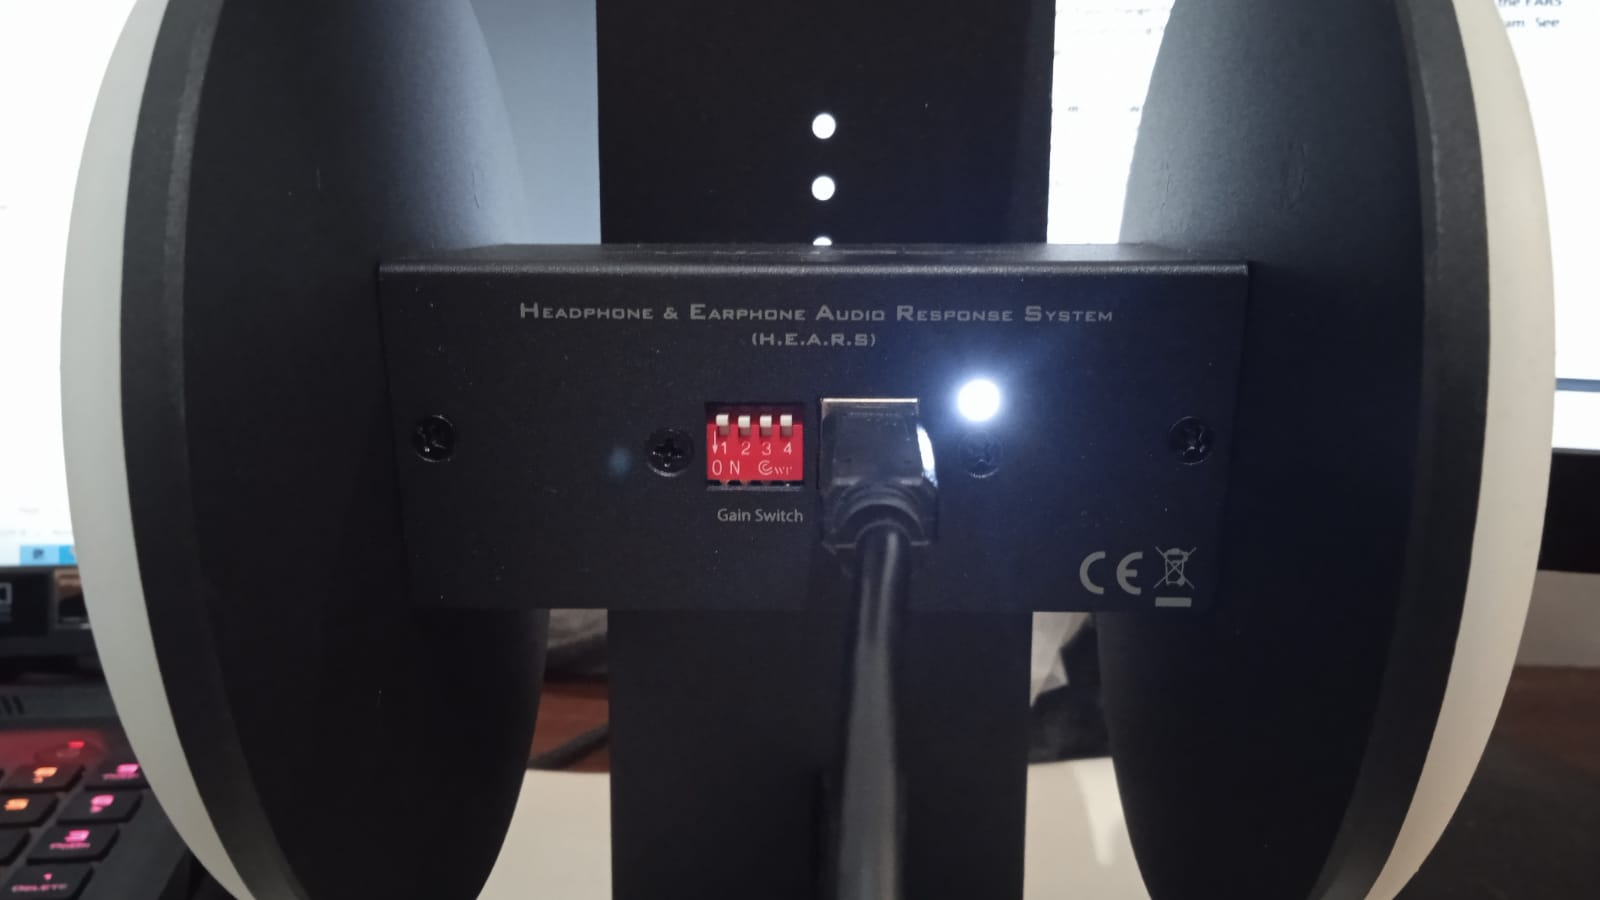
\includegraphics[width=\textwidth]{images/plug-in}
				\caption{}
			\end{subfigure}
			\begin{subfigure}[]{.45\textwidth}
				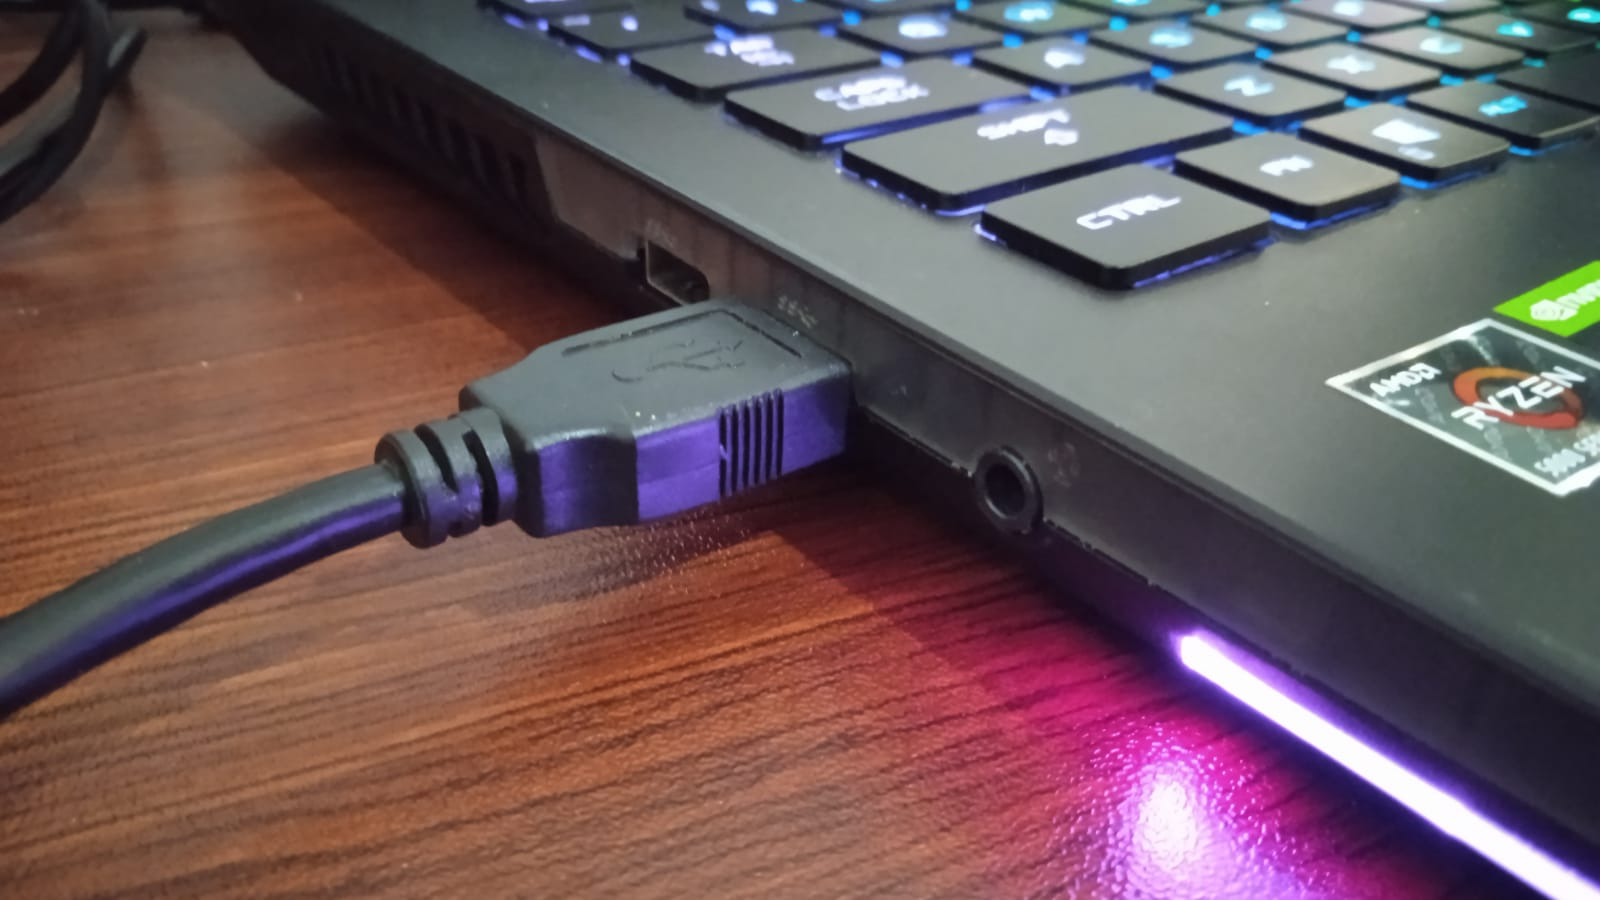
\includegraphics[width=\textwidth]{images/plug-in-usb}
				\caption{}
			\end{subfigure}
			\caption{Sambungan pada (a) miniDSP EARS dan (b) laptop}
			\label{fig:plug-in}
		\end{figure}

		\begin{figure}[H]
			\centering
			\begin{subfigure}[]{.45\textwidth}
				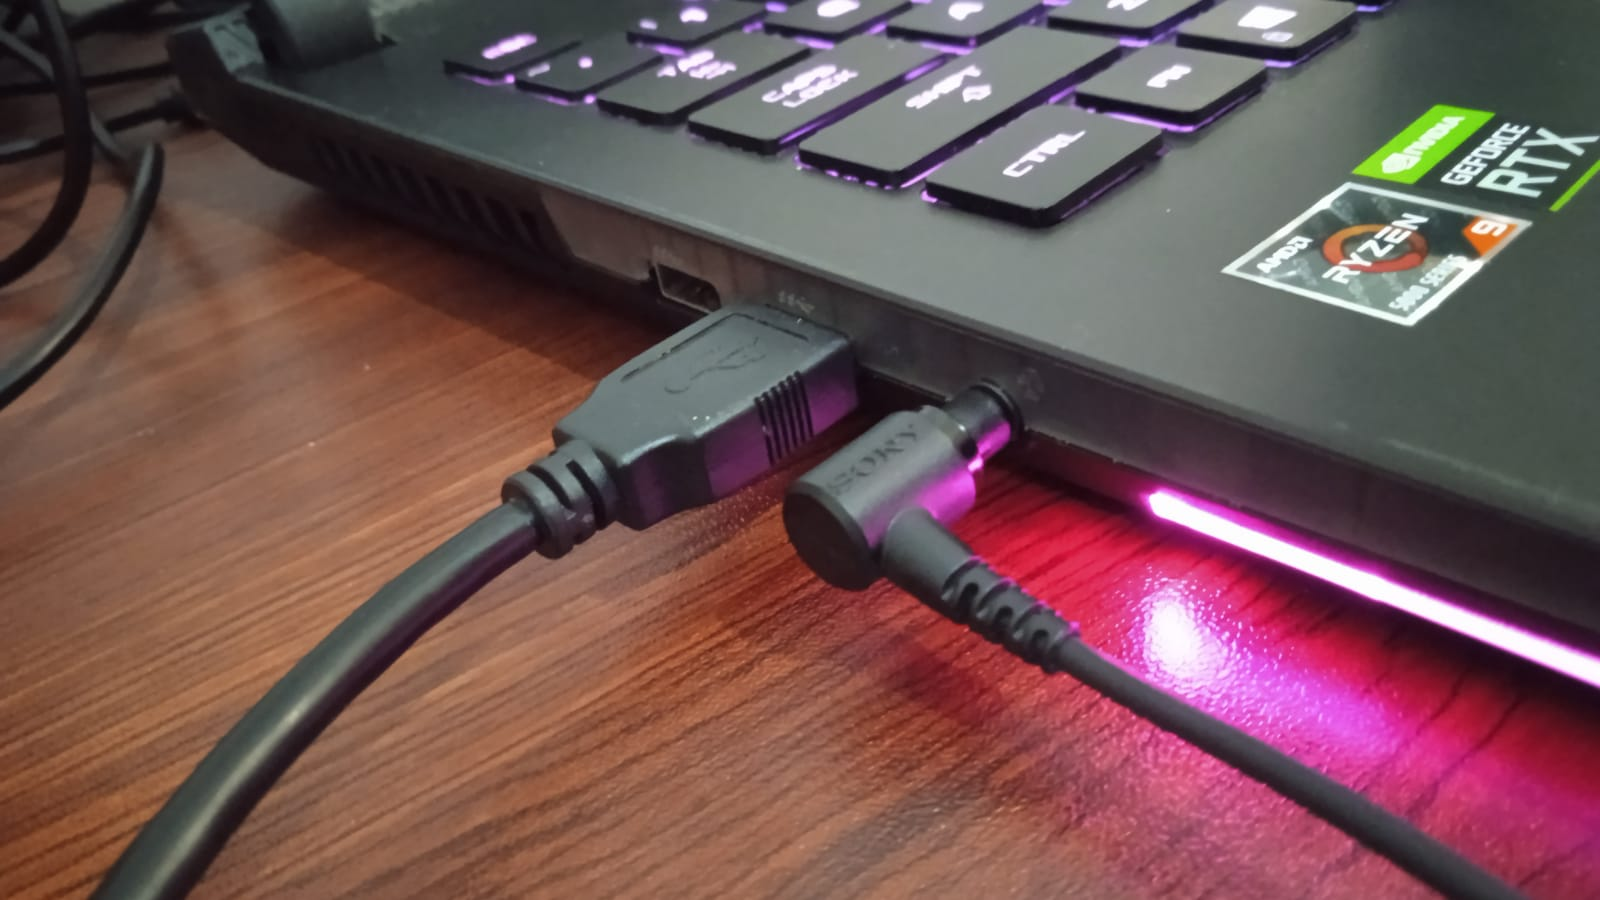
\includegraphics[width=\textwidth]{images/plug-in-audio}
				\caption{}
			\end{subfigure}

			\begin{subfigure}[]{.45\textwidth}
				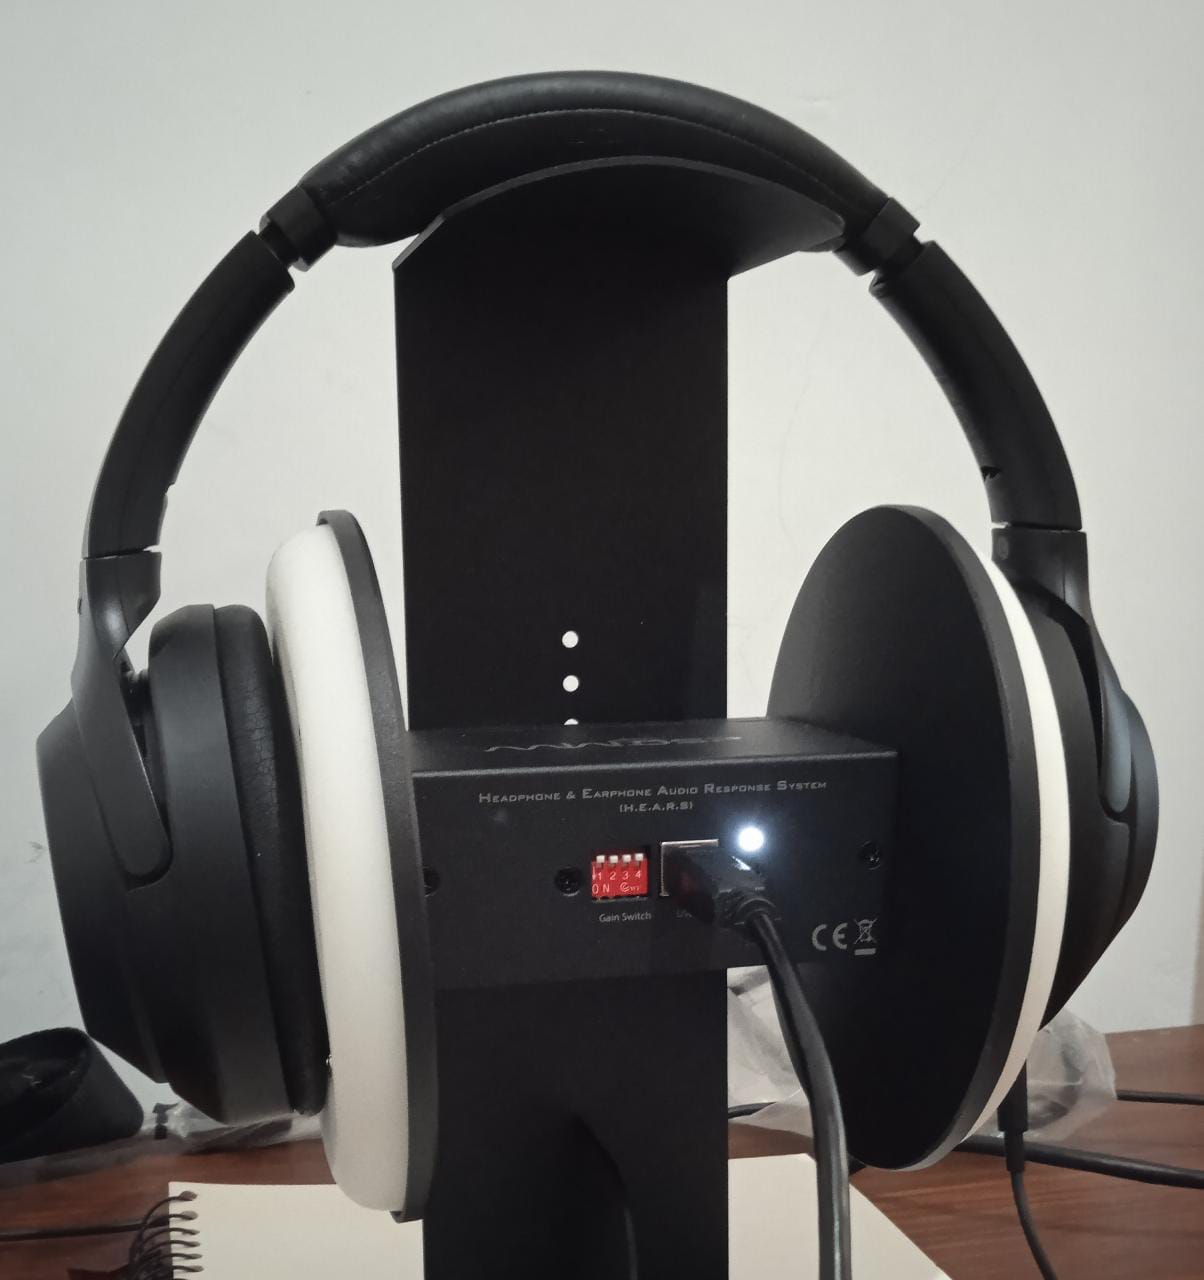
\includegraphics[width=\textwidth]{images/headphone-mounted}
				\caption{}
			\end{subfigure}
			\caption{Konfigurasi (a) sambungan headphone pada laptop, dan kemudian (b) headphone diletakkan pada miniDSP EARS}
			\label{fig:headphone-mounting}
		\end{figure}

		\item Hubungkan headphone dengan laptop menggunakan sambungan kabel (untuk wired headphone) atau koneksi bluetooth (untuk wireless headphone). Letakkan headphone pada miniDSP EARS seperti pada Gambar \ref{fig:headphone-mounting}. Pastikan posisi headphone sesuai dengan daun telinga pada miniDSP EARS.


	\end{enumerate}

	\subparagraph{Kalibrasi miniDSP EARS}
	\label{subparagraph:kalibrasi}
	\begin{enumerate}
		\item Unduh dokumen kalibrasi miniDSP EARS halaman \href{https://www.minidsp.com/products/acoustic-measurement/ears-headphone-jig}{unduhan}. Masukkan serial number dari perangkat (terdapat pada bagian panel bawah perangkat) untuk mengakses file unduhan.

		\item Pilih file kalibrasi yang sesuai dengan kondisi/mode pengujian yang dilakukan.

		\item Atur setup dan pengaturan perangkat sesuai dengan penejelasan pada bagian \ref{setup}

		\item Pastikan nilai sample rate dari perangkat input (miniDSP EARS) dan output (headphone) memiliki nilai yang sama.
		\begin{itemize}
			\item Pengecekan sample rate pada input dapat dilakukan melalui {\bf Control Panel} $\rightarrow$ {\bf Hardware and Sound} $\rightarrow$ {\bf Manage Audio Devices} $\rightarrow$ {\bf Input Device} $\rightarrow$ {\bf Properties} $\rightarrow$ {\bf Advanced}.
			\item Pengecekan sample rate pada output dapat dilakukan melalui {\bf Control Panel} $\rightarrow$ {\bf Hardware and Sound} $\rightarrow$ {\bf Manage Audio Devices} $\rightarrow$ {\bf Output Device} $\rightarrow$ {\bf Properties} $\rightarrow$ {\bf Advanced}.
		\end{itemize}

		\item Buka software REW (tampilan awal software seperti pada Gambar \ref{fig:rew-initial}). Tampilan dialog akan muncul menunjukkan perangkat miniDSP EARS terbaca oleh laptop. Tekan {\bf Yes}.

		\begin{figure}[H]
			\centering
			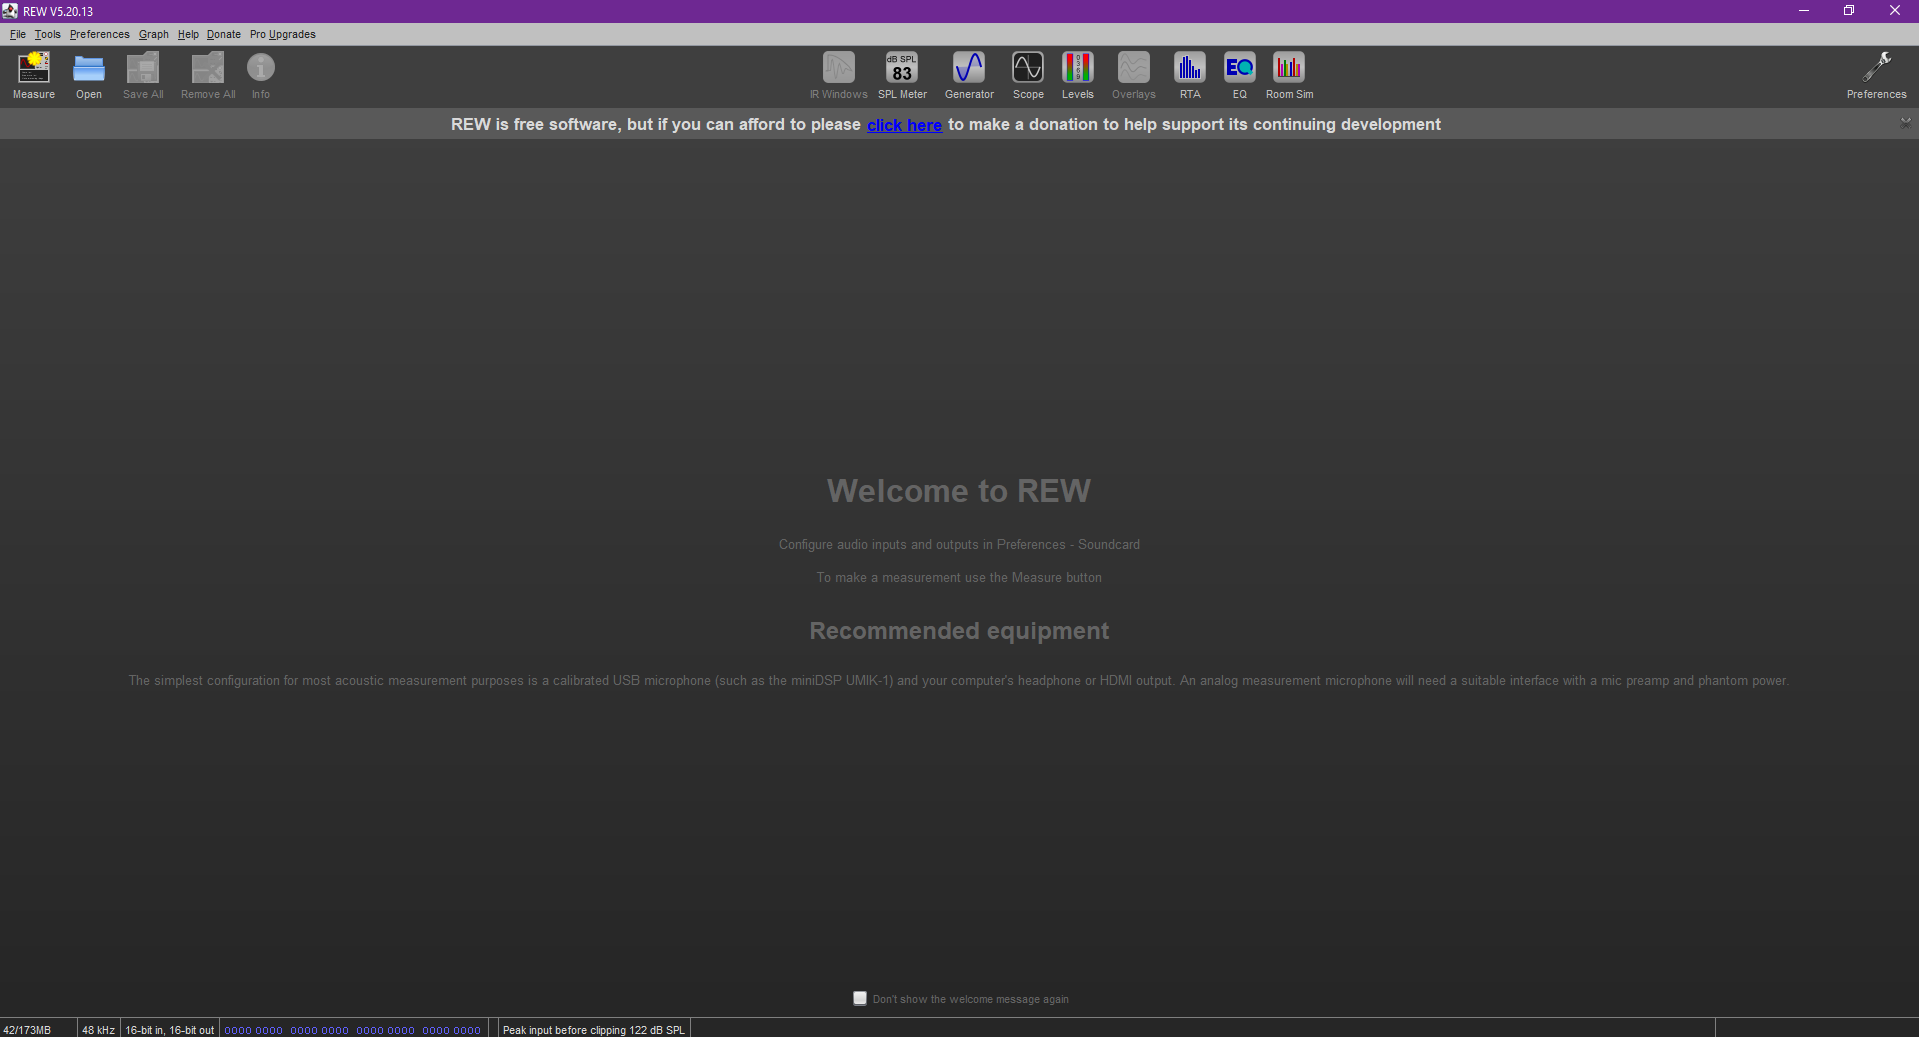
\includegraphics[width=0.6\textwidth]{images/rew-initial}
			\caption{Tampilan awal software REW}
			\label{fig:rew-initial}
		\end{figure}

		\item Tampilan dialog muncul menanyakan apakah file kalibrasi telah tersedia. Tekan {\bf Yes}.

		\item Unggah file kalibrasi yang akan digunakan, masing-masing untuk channel kiri dan kanan.

		\item Jika dialog pada langkah 5-6 tidak muncul, maka langsung buka menu {\bf Preferences}.

		\item Buka menu {\bf Preferences}. Pada tab Soundcard, pastikan nilai sample rate, output device, dan input device menunjukkan pengaturan seperti pada Gambar \ref{fig:rew-preferences}.

		\begin{figure}[H]
			\centering
			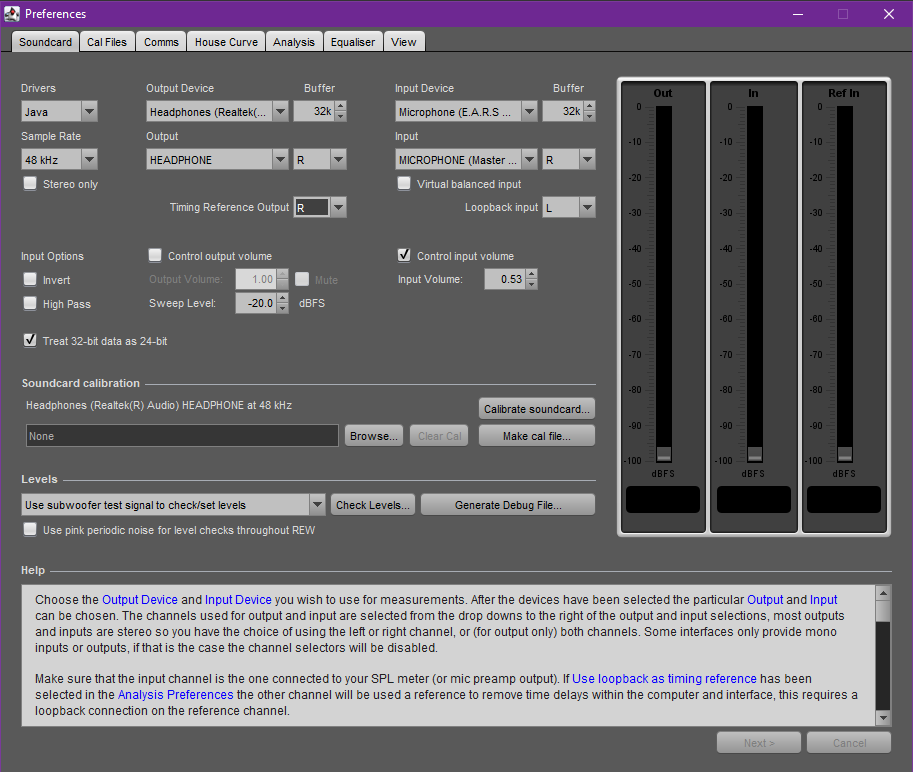
\includegraphics[width=0.6\textwidth]{images/rew-preferences}
			\caption{Tampilan menu Preferences software REW}
			\label{fig:rew-preferences}
		\end{figure}

		\item Buka tab {\bf Cal Files}. Pastikan file kalibrasi sudah terunggah (Gambar \ref{fig:rew-cal}).

		\begin{figure}[H]
			\centering
			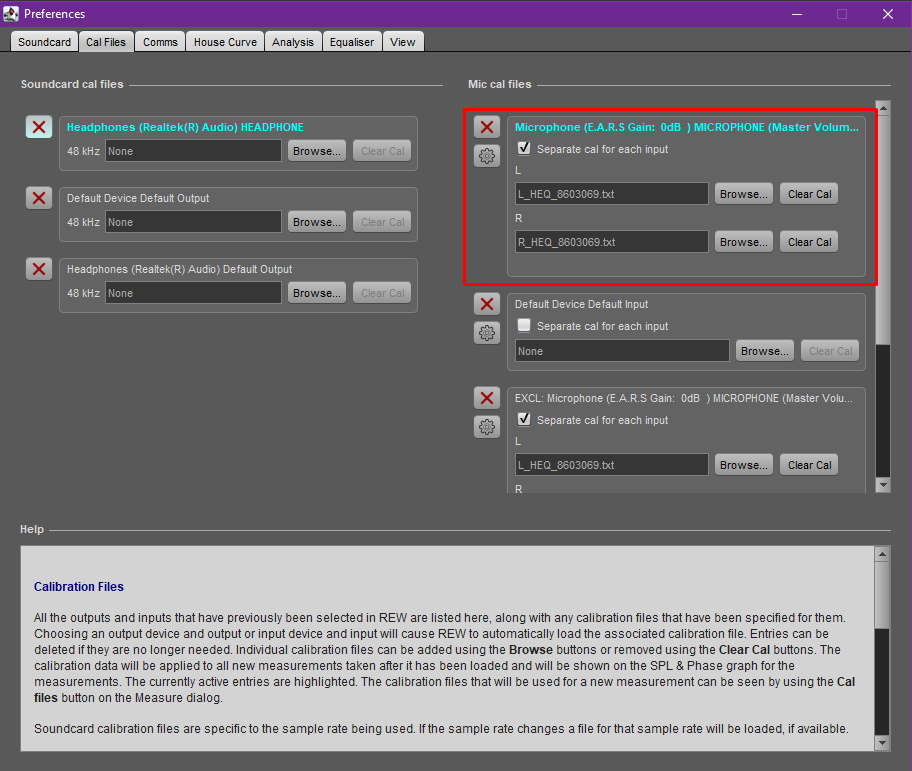
\includegraphics[width=0.6\textwidth]{images/rew-calibration}
			\caption{Tampilan menu Preferences software REW}
			\label{fig:rew-cal}
		\end{figure}

		\item Kembali ke menu utama. Buka menu {\bf Generator} (Gambar \ref{fig:rew-generator}). Pilih tab {\bf Tones} dan {\bf Sine}. Atur nilai frekuensi menjadi 300 Hz dan nilai RMS level sebesar -20.00 dB FS. Tekan tombol {\bf Play} pada bagian kanan bawah.

		\begin{figure}[H]
			\centering
			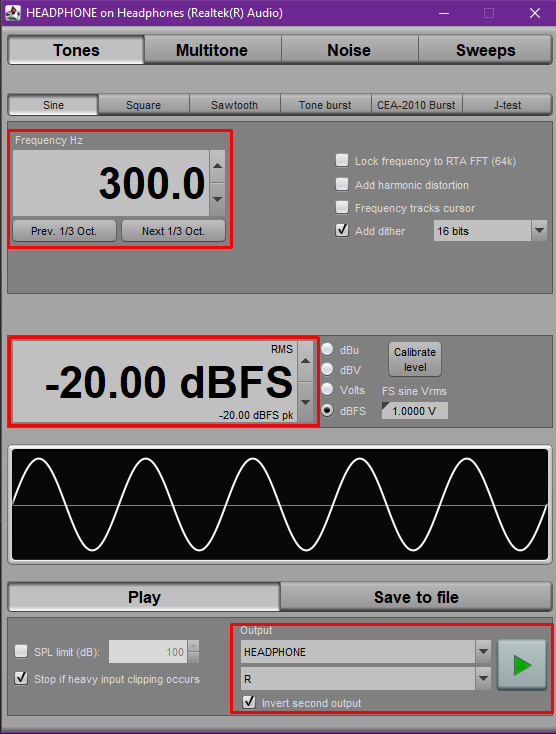
\includegraphics[width=0.4\textwidth]{images/rew-generator}
			\caption{Tampilan menu Preferences software REW}
			\label{fig:rew-generator}
		\end{figure}

		\item Buka menu {\bf SPL Meter} (Gambar \ref{fig:rew-spl-meter}). Atur volume pada headphone hingga mencapai nilai 84 dB. Nilai volume dapat diatur lebih tinggi, namun pastikan hal tersebut tidak melebihi batas kemampuan headphone.

		\begin{figure}[H]
			\centering
			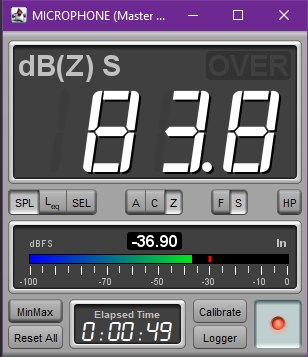
\includegraphics[width=0.4\textwidth]{images/rew-splmeter}
			\caption{Tampilan menu Preferences software REW}
			\label{fig:rew-spl-meter}
		\end{figure}

		\item Kembali ke menu {\bf Generator}. Tekan tombol {\bf Stop} pada bagian kanan bawah. Tutup menu {\bf Generator} dan {\bf SPL Meter}.

	\end{enumerate}

	\subparagraph{Pengukuran dan Pengambilan Data}
	\begin{enumerate}
		\item Buka menu {\bf Measure} pada REW, lakukan pengaturan sesuai pada Gambar \ref{fig:rew-measurement-left}. Pilih tab {\bf SPL}, atur nilai range frekuensi mulai 20-20.000 Hz. Atur nilai level pada -20.00 dB FS. Kemudian pilih tab {\bf Sweep}. Pastikan channel aktif dari device output dan input adalah sisi kiri (left). Tekan {\bf Start} untuk memulai pengukuran.

		\begin{figure}[H]
			\centering
			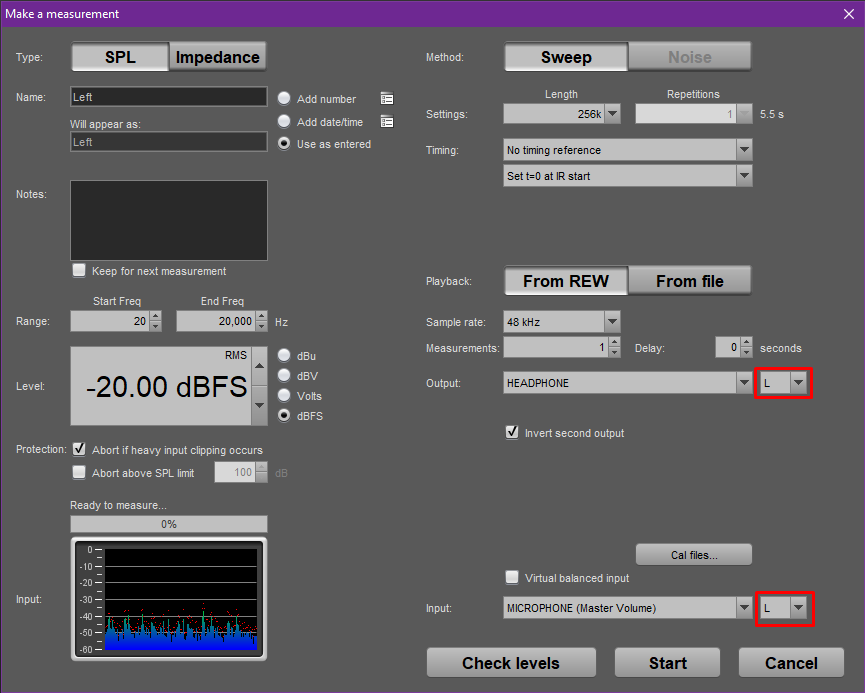
\includegraphics[width=0.8\textwidth]{images/rew-measurement-L}
			\caption{Tampilan menu Preferences software REW}
			\label{fig:rew-measurement-left}
		\end{figure}

		\item Lakukan pengukuran selanjutnya dengan mengubah channel input dan output ke sisi kanan (right), seperti ditunjukkan pada Gambar \ref{fig:rew-measurement-right}. Tekan {\bf Start} untuk memulai pengukuran.

		\begin{figure}[H]
			\centering
			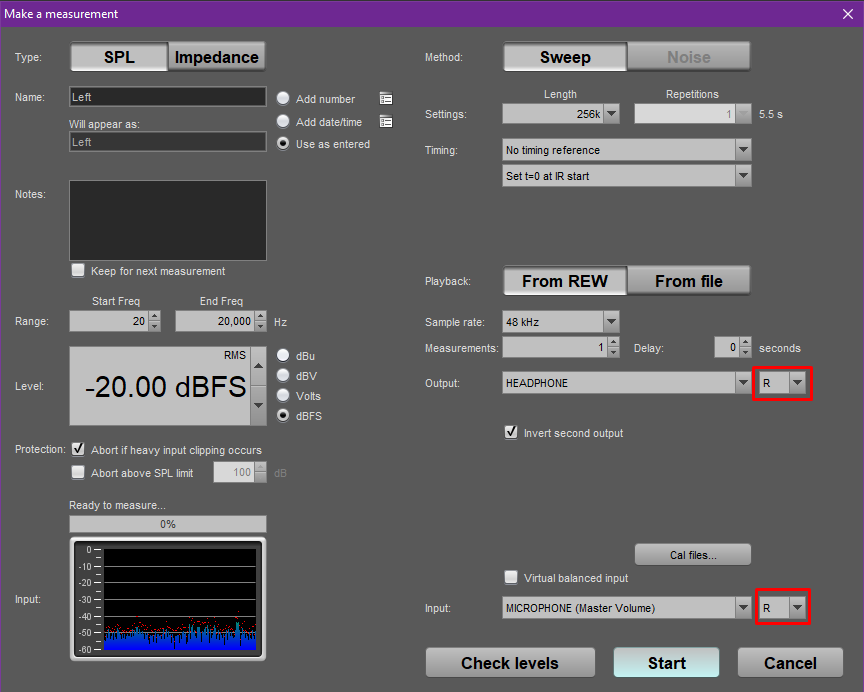
\includegraphics[width=0.8\textwidth]{images/rew-measurement-R}
			\caption{Tampilan menu Preferences software REW}
			\label{fig:rew-measurement-right}
		\end{figure}

		\item Pilih menu {\bf Overlay} untuk menampilkan hasil untuk kedua channel sekaligus. Tampilan contoh hasil pengukuran nilai frequency response dan distortion ditunjukkan berturut-turut pada Gambar \ref{fig:rew-overlay} dan Gambar \ref{fig:rew-overlay-distortion}.

		\begin{figure}[H]
			\centering
			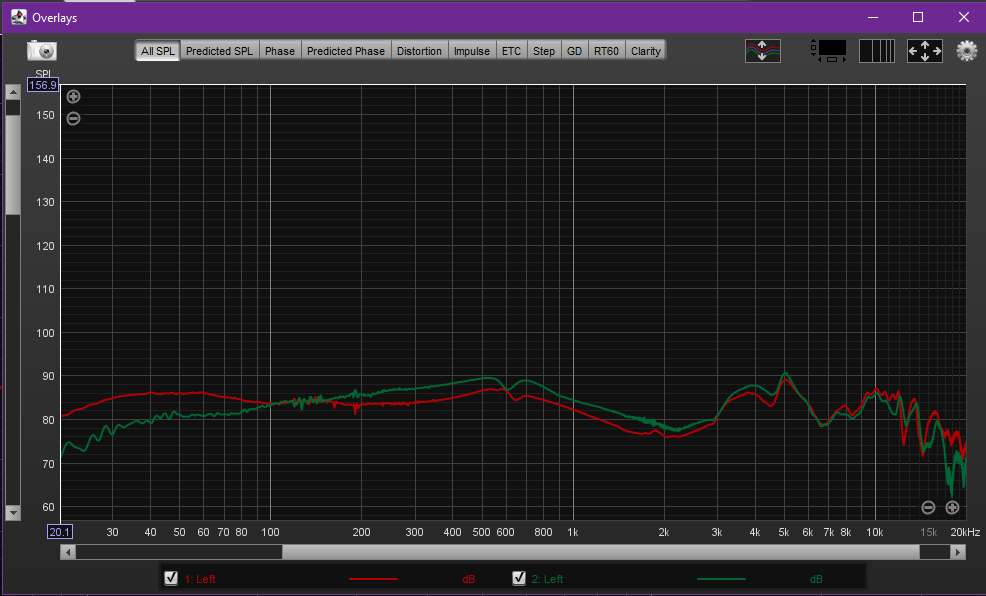
\includegraphics[width=0.8\textwidth]{images/rew-overlay}
			\caption{Tampilan menu Preferences software REW}
			\label{fig:rew-overlay}
		\end{figure}

		\begin{figure}[H]
			\centering
			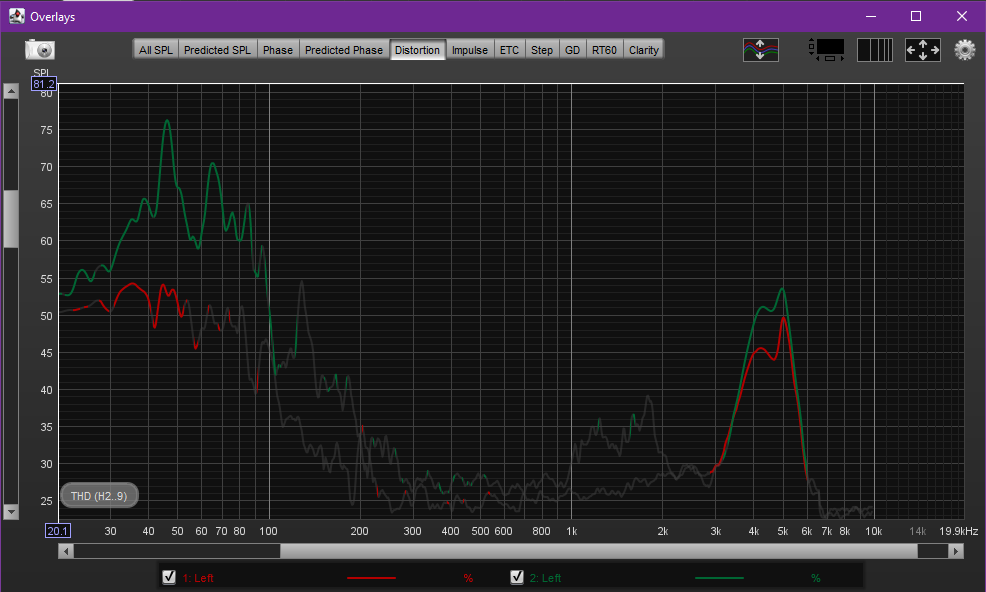
\includegraphics[width=0.8\textwidth]{images/rew-overlay-distortion}
			\caption{Tampilan menu Preferences software REW}
			\label{fig:rew-overlay-distortion}
		\end{figure}

		\item Simpan hasil pengukuran yang dilakukan pada tab {\bf File} $\rightarrow$ {\bf Save as}.

		\item Prosedur pengujian yang sama dilakukan untuk jenis headphone lain yang digunakan pada pengujian ini.

	\end{enumerate}

	\paragraph{Pengukuran Nilai SPL Luaran Tone Audiometer Portabel}
	\subparagraph{Setup dan Pengaturan Perangkat}
		\begin{enumerate}
			\item Pasang Headphone pada unit EARS sebagaimana jika digunakan pada telinga manusia.
			Pastikan kiri dan kanan tidak terbalik.
			Pastikan Headphone menutup lubang telinga.

			\begin{figure}[H]
				\centering
				\begin{subfigure}[H]{0.4\textwidth}
					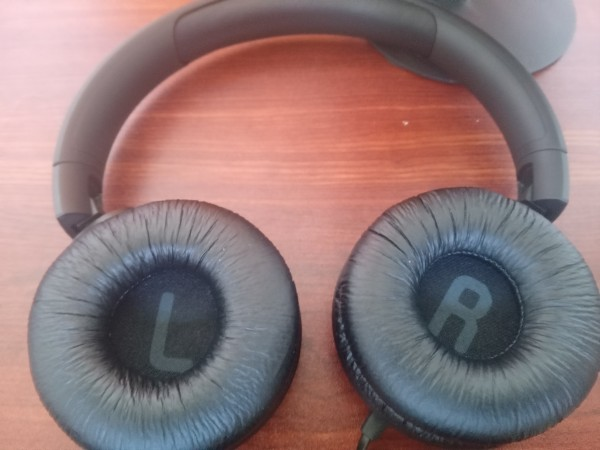
\includegraphics[width=\textwidth]{images/pasang/chjbl}
					\caption{Label Channel}
				\end{subfigure}
				\begin{subfigure}[H]{0.4\textwidth}
					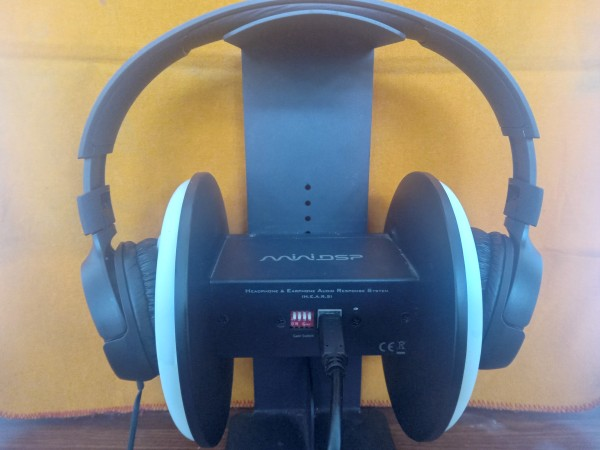
\includegraphics[width=\textwidth]{images/pasang/pasangjbl}
					\caption{Pasang Headphone}
				\end{subfigure}
%				\\
%				\begin{subfigure}[H]{0.3\textwidth}
%					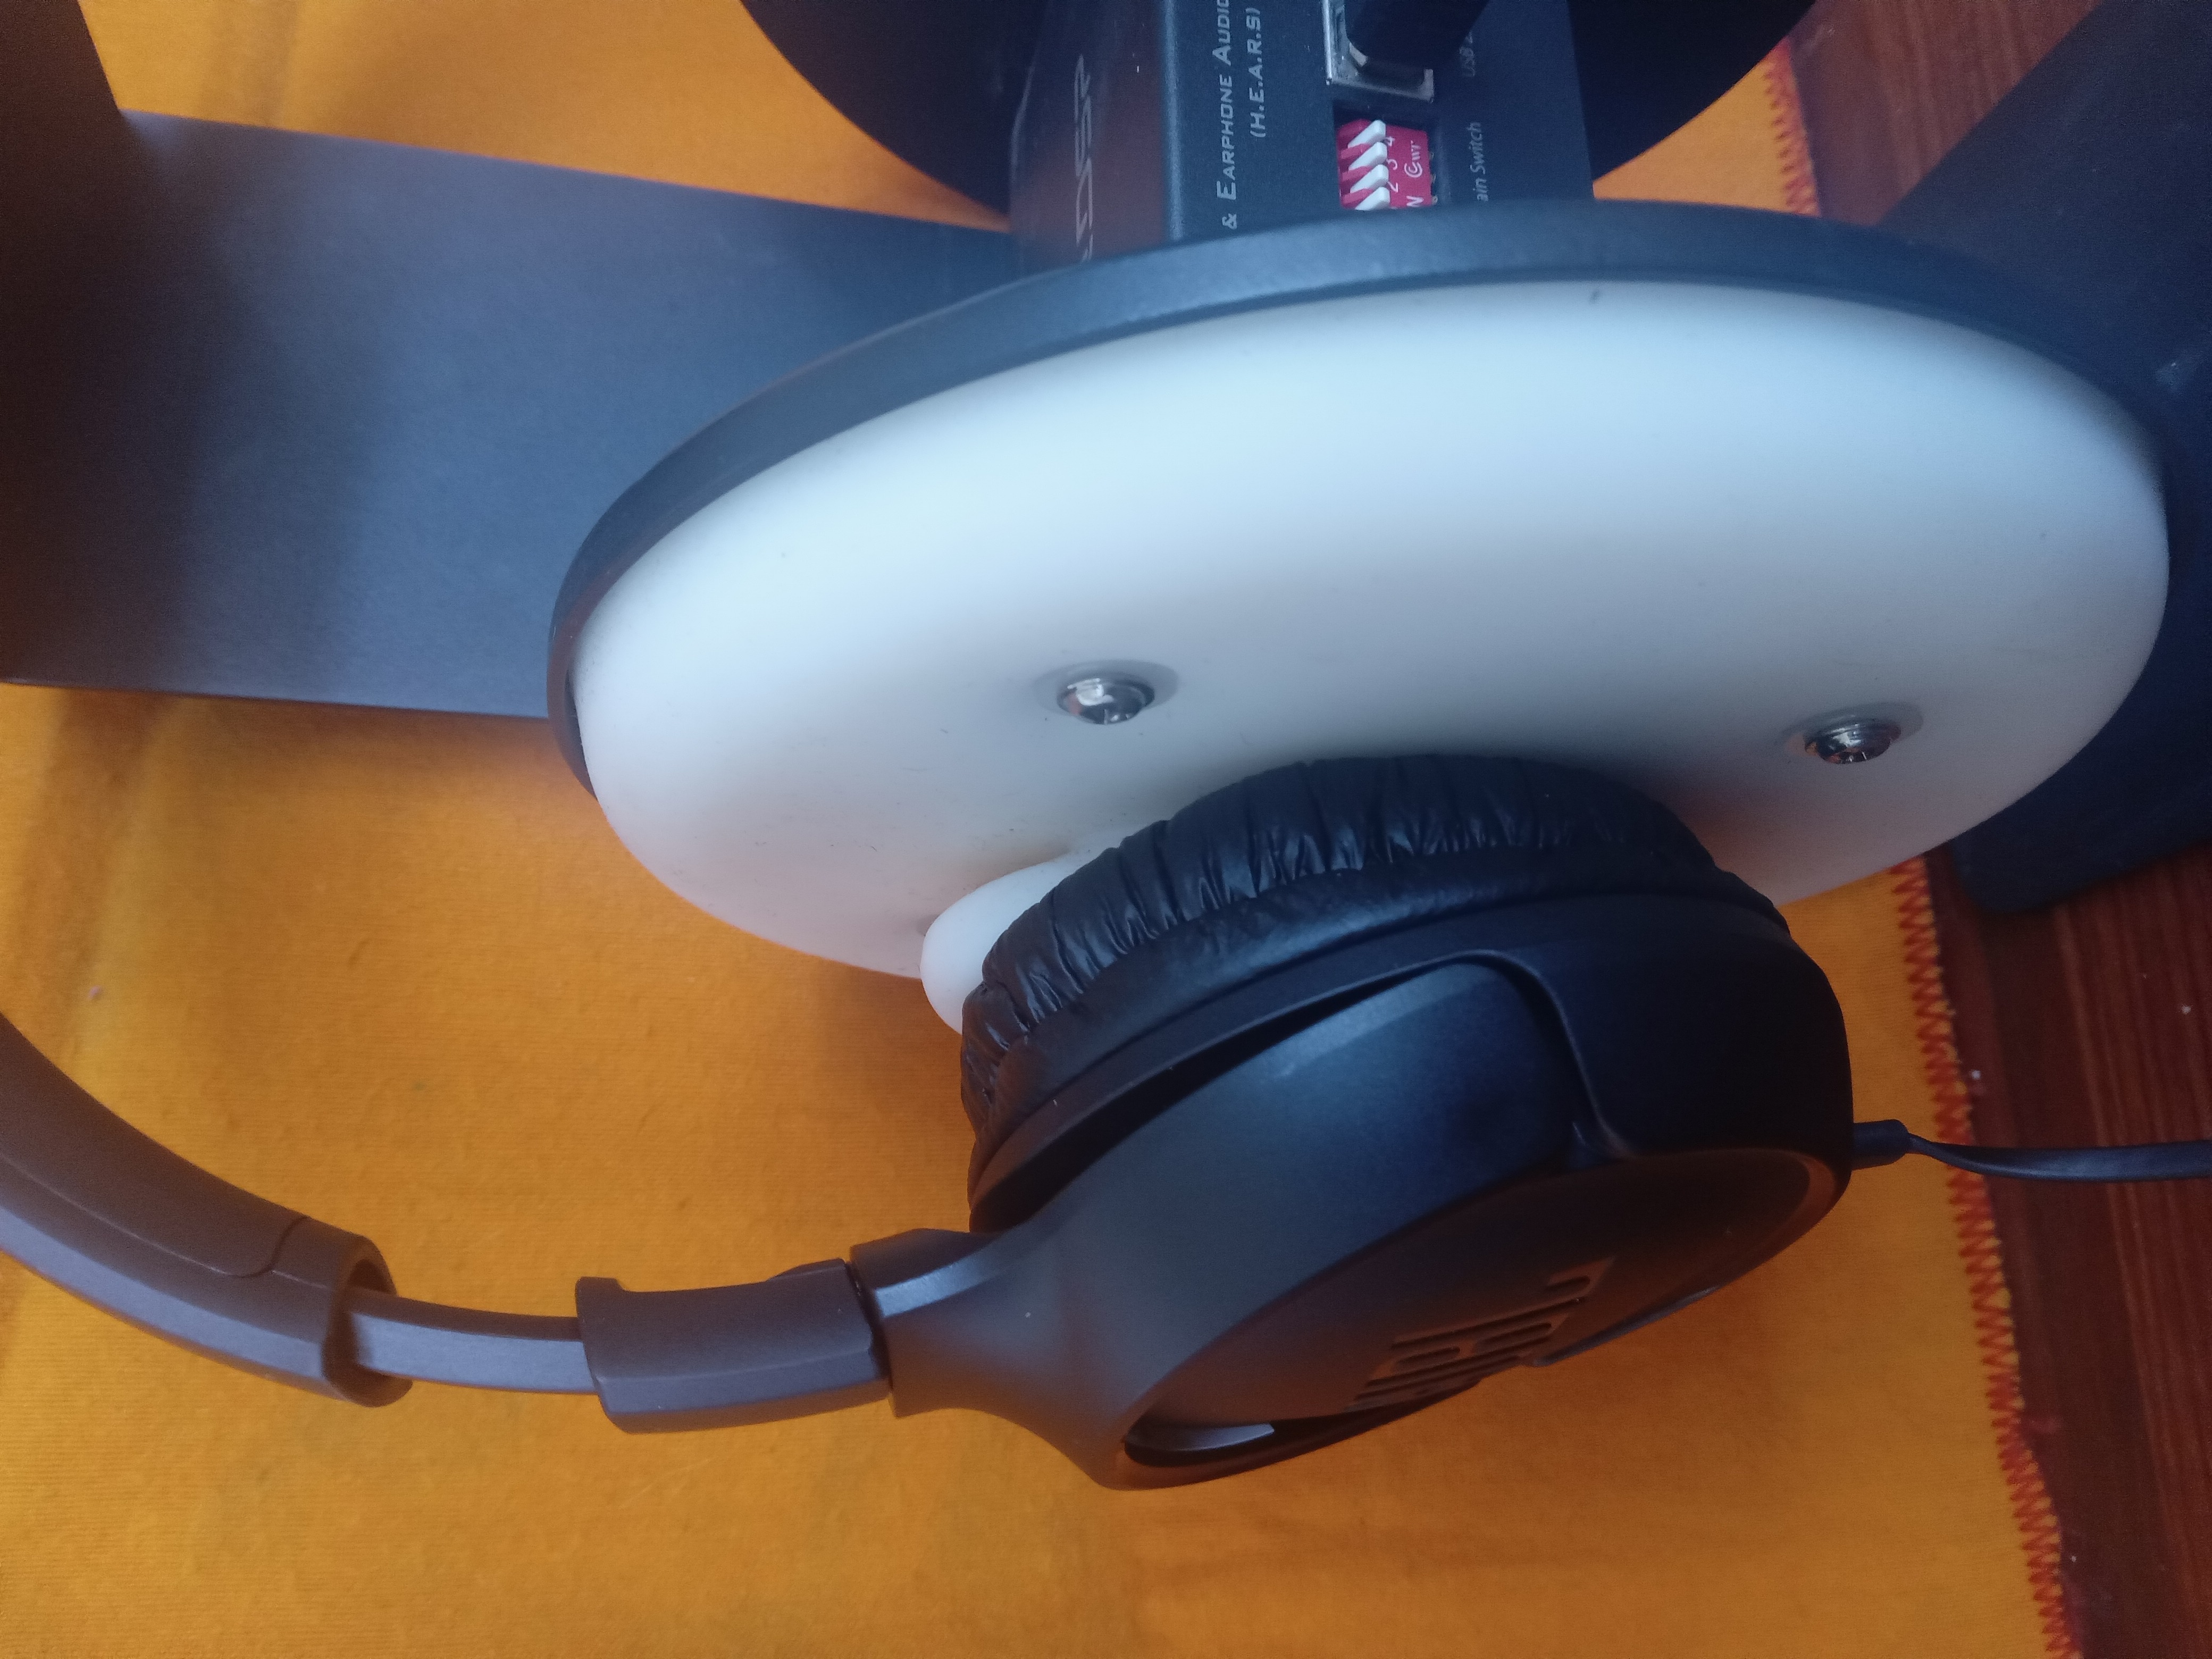
\includegraphics[width=\textwidth,angle=-90]{images/pasang/tutupjbl}
%					\caption{Menutup Telinga}
%				\end{subfigure}

				\caption{Pemasangan Headphone pada EARS}
			\end{figure}

			\item Sambung Jack Audio Headphone ke Konsol
			\begin{figure}[H]
				\centering
				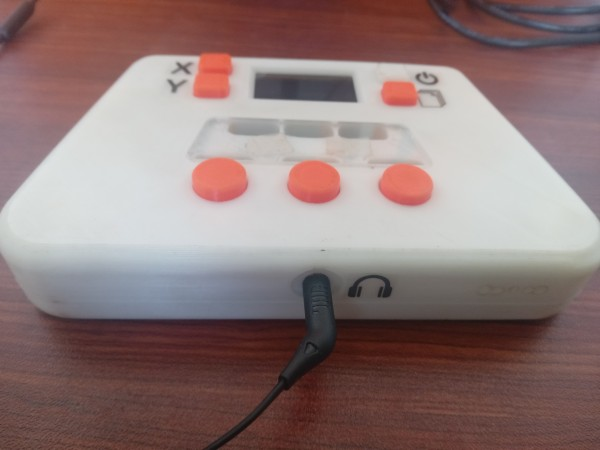
\includegraphics[width=200pt]{images/pasang/sambung_audio}
				\caption{Sambung Jack Audio}
			\end{figure}

			\item Nyalakan Unit. Tunggu hingga LED biru berkedip.
			\begin{figure}[H]
				\centering
				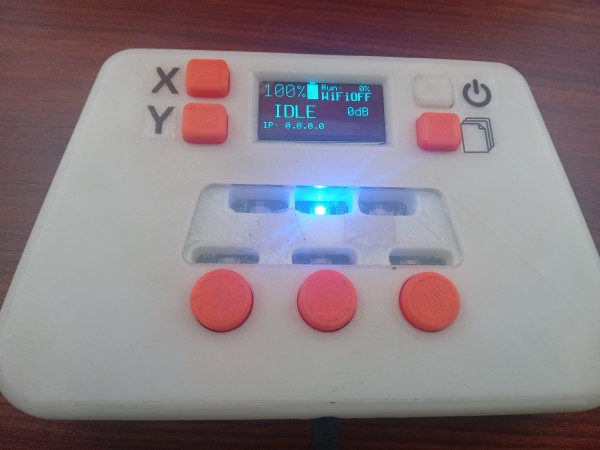
\includegraphics[width=200pt]{images/pasang/nyalakan_unit}
				\caption{Nyalakan Unit}
			\end{figure}
			\item Sambung Kabel USB ke Konsol
			\begin{figure}[H]
				\centering
				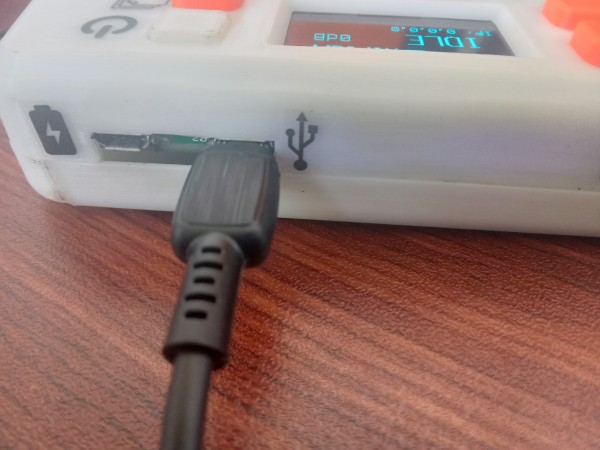
\includegraphics[width=200pt]{images/pasang/sambung_usb}
				\caption{Sambung Kabel USB}
			\end{figure}
		\end{enumerate}

	\subparagraph{Komunikasi Serial}

	\begin{enumerate}
		\item Berikut adalah perangkat lunak komunikasi serial ke Konsol yang perlu disiapkan untuk pengujian ini (panduan ini menggunakan Windows-7 32-bit sebagai contoh)

		\item Install driver ARM USB-CDC.\\
		Untuk dapat menghubungkan unit prototype dengan komputer,
		diperlukan driver ARM USB-CDC untuk komunikasi serial.

		\begin{itemize}
			\item File installer (sesuaikan dengan bit OS).
			Dapat didownload di \href{https://drive.google.com/drive/folders/19gXVrxR68SFHQUGGGgKb0Da03oV7Rh41?usp=share_link}{USB-CDC\_Driver}.
			\begin{figure}[H]
				\centering
				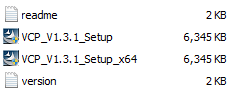
\includegraphics[width=200pt]{images/software/driver}
				\caption{Installer Driver}
			\end{figure}

			\item Instalasi driver (tanpa unit prototype terhubung) cukup mudah sebagaimana umumnya.
			\begin{figure}[H]
				\centering
				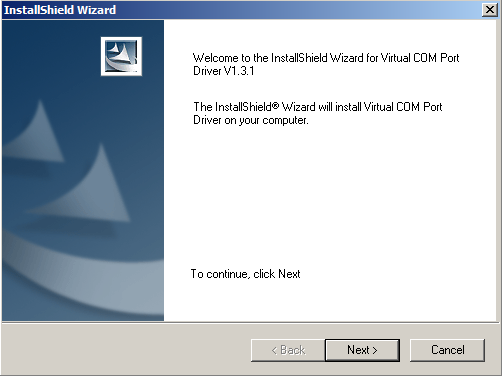
\includegraphics[width=200pt]{images/software/install_driver}
				\caption{Mulai instal driver}
			\end{figure}
		\end{itemize}

		\item Sambungkan unit prototype yang telah nyala dengan komputer via kabel USB.
		\begin{figure}[H]
			\centering
			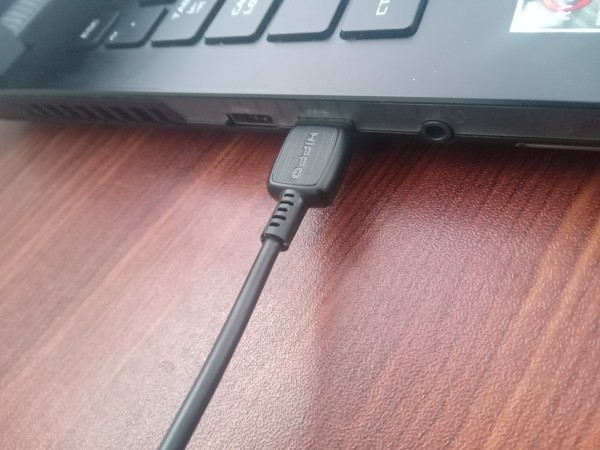
\includegraphics[width=200pt]{images/pasang/laptop_usb}
			\caption{Sambung Kabel USB ke Laptop}
		\end{figure}

		\item Tunggu hingga driver selesai mengkonfigurasi otomatis

		\item Cek \textit{Device Manager} untuk mengetahui Nomor Serial-Port
		\begin{itemize}
			\item Buka run-command dialog dengan kombinasi keyboard %(\keys{\WinKey + r})

			\item masukkan perintah \textbf{devmgmt.msc}.
			\begin{figure}[H]
				\centering
				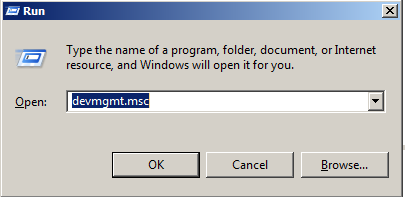
\includegraphics[width=200pt]{images/software/devicemgr}
				\caption{Memanggil Device Manager}
			\end{figure}

			\item Tekan (\keys{\return}) atau klik OK

			\item Cari entry \textit{Ports (COM and LPT)}.
			Catat nomor port untuk entry \textit{STMicroelectronics Virtual COM Port}.
			Dalam contoh ini, terkonfigurasi pada COM3.

			\begin{figure}[H]
				\centering
				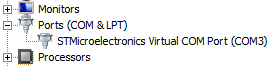
\includegraphics[width=200pt]{images/software/comport}
				\caption{Serial Komunikasi pada COM3}
			\end{figure}
		\end{itemize}


		\item Install Serial Terminal.
		Untuk dapat berkomunikasi via serial port, perlu diinstall serial terminal.
		Disini dicontohkan menggunakan \textit{Hercules}.

		\begin{itemize}
			\item Program terminal Hercules. Dapat didownload di \href{https://drive.google.com/drive/folders/1fgNPnGeSm20TrFfwmeCa4B24WIN_t_o_?usp=share_link}{Terminal}.
			\begin{figure}[H]
				\centering
				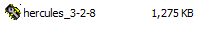
\includegraphics[width=200pt]{images/software/hercules}
				\caption{Hercules Terminal}
			\end{figure}

			\item Jalankan program Hercules.
			Jika muncul konfirmasi lisensi, cukup \textit{Close} saja.

			\item Pilih tab \textit{Serial}.
			\begin{figure}[H]
				\centering
				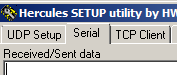
\includegraphics[width=200pt]{images/software/hercules_serial}
				\caption{Serial Terminal}
			\end{figure}
		\end{itemize}

		\item Test Komunikasi Serial
		\begin{itemize}
			\item Hercules Serial Terminal
			\begin{figure}[H]
				\centering
				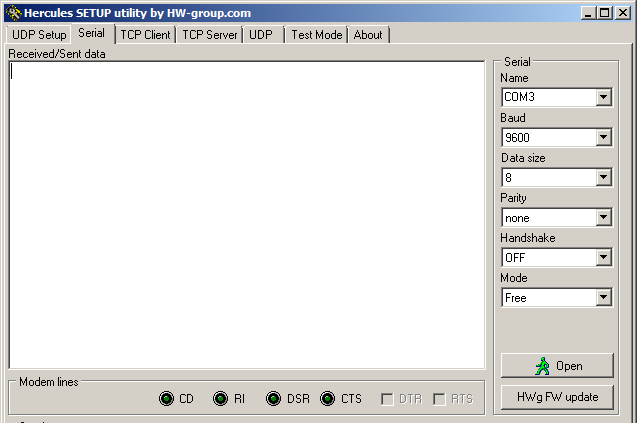
\includegraphics[width=250pt]{images/software/hercules_terminal}
				\caption{Hercules Serial Terminal}
			\end{figure}

			\item Setting Port pada Serial Terminal sebagai berikut
			\begin{itemize}
				\item Name     : COM3
				\item Baud     : 9600
				\item Data size: 8
				\item Parity   : none
			\end{itemize}

			\begin{figure}[H]
				\centering
				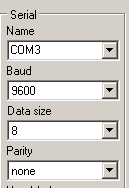
\includegraphics[width=100pt]{images/software/hercules_port}
				\caption{Pengaturan serial port}
			\end{figure}

			\item Klik Open (pastikan unit prototype sudah standby dan terhubung
			serta nama COM port sudah sesuai)

			\begin{figure}[H]
				\centering
				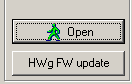
\includegraphics[width=100pt]{images/software/hercules_open}
				\caption{Open Serial Port}
			\end{figure}

			\item Kolom terminal akan menampilkan pesan:
			\begin{minted}[frame=lines,framesep=2mm,fontsize=\small]{text}
Serial port COM3 opened
			\end{minted}

			\item Selanjutnya, pada kolom terminal,
			masukkan perintah berikut dan diakhiri dengan (\keys{\return})
			\begin{minted}[frame=lines,framesep=2mm,fontsize=\small]{text}
info
			\end{minted}
			Serial akan menampilkan informasi kernel dan platform
			\begin{figure}[H]
				\centering
				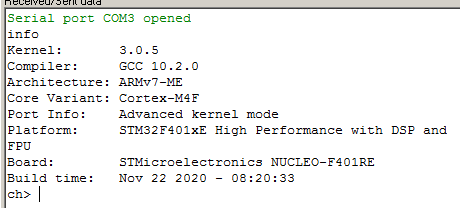
\includegraphics[width=300pt]{images/software/hercules_text}
				\caption{Informasi Platform}
			\end{figure}
		\end{itemize}

	\end{enumerate}

	Berikut beberapa contoh perintah serial yang dapat diakses melalui komunikasi serial Konsol:

	\begin{table}[H]
		\renewcommand{\tablename}{Tabel}
		\centering
		\caption{Contoh perintah serial yang tersedia pada konsol Audiometri. \label{table:serial-code}}
		\begin{tabular}{| p{0.05\textwidth} | p{0.1\textwidth} | p{0.15\textwidth} | p{0.1\textwidth} | p{0.5\textwidth} |}
			\hline
			\textbf{No} & \textbf{Perintah} & \textbf{Fungsi} & \textbf{Contoh Perintah} & \textbf{Contoh Respon} \\
			\hline
			1 & \textit{coba} & Menguji Respon Serial & \textit{test} & \textit{Serial Console at 9600 \& buffer size 8 bit} \\
			\hline
			2 & \textit{help} & Menampilkan Perintah yang tersedia & \textit{help} & \textit{coba mmc out tes led sig tone virt ...} \\
			\hline
			3 & \textit{info} & Menampilkan Info Platform Chip & \textit{info} & \textit{Kernel: 6.1.4Compiler: GCC 12.1.0 ...} \\
			\hline
			4 & \textit{mmc} & Mengelola isi SDCard & \textit{mmc} & \textit{usage: mmc [test|ls|lsnum| ...} \\
			& & & \textit{mmc ls} & \textit{HT1.TXT HT2.TXT ...} \\
			& & & \textit{mmc cat 1} & \textit{\{"audiogram":\{ ...} \\
			\hline
			5 & \textit{out} & Menghasilkan nada murni &  \textit{out} & \textit{usage: out <0/1> <freq> <ampl> ...} \\
			& & & \textit{out 500 11} & \textit{Out: Freq:  500 Ampl:11} \\
			& & & \textit{out 1 250 8} & \textit{Out: Freq:  250 Ampl:8} \\
			\hline
		\end{tabular}
	\end{table}

	\textbf{Keterangan}: Beberapa keterangan perintah \textit{out}:
	\begin{itemize}
		\item Pilihan Channel adalah 0 atau kosong untuk kiri, dan 1 untuk kanan.
		\item Pilihan Frekuensi Nada Murni: 250Hz, 500Hz, 1000Hz, 2000Hz, 4000Hz, dan 8000Hz.
		\item Pilihan Skala Loudness Nada Murni: 1, 2, 3, 4, 5, 6, 7, 8, 9, 10, dan 11.
	\end{itemize}

	\subparagraph{Pengukuran dan Pengambilan Data}

		\begin{enumerate}
			\item Pengujian yang dimaksudkan untuk mendapatkan nilai aktual output audio nada murni dalam satuan dBA.

			\item Output nada murni memiliki karakteristik:
			\begin{itemize}
				\item frekuensi adalah nilai frekuensi (dalam Hz) yaitu 250, 500, 1000, 2000, 4000, dan 8000.
				\item amplitudo adalah skala amplitudo antara 1 sampai 11.
			\end{itemize}

			\item Berikut contoh perintah untuk menghasilkan nada murni (sebagaimana Tabel \ref{table:serial-code}):

			\begin{itemize}
				\item Nada murni pada frekuensi 500Hz dan skala 11.
				\begin{minted}[frame=lines,framesep=2mm,fontsize=\small]{text}
out 500 11
				\end{minted}

				\item Nada murni pada frekuensi 500Hz dan skala 1.
				\begin{minted}[frame=lines,framesep=2mm,fontsize=\small]{text}
out 500 1
				\end{minted}

				\item Nada murni pada frekuensi 500Hz dan skala 11 di channel/sisi kanan.
				\begin{minted}[frame=lines,framesep=2mm,fontsize=\small]{text}
out 1 500 11
				\end{minted}

				\textbf{Catatan:} Pengukuran dua sisi diperlukan jika diasumsikan headphone berbeda karakteristik kedua sisinya.
			\end{itemize}

			\item Buka terminal serial dan software REW. Pada software REW, lakukan prosedur kalibrasi sesuai pada bagian \ref{subparagraph:kalibrasi}.

			\item Pada software REW, buka menu {\bf RTA}. Atur pengaturan dengan menekan simbol {\bf Setting} pada bagian kanan atas menu. Atur mode display RTA mengikuti Gambar.

			\item Siapkan perangkat audiometer portable. Pada terminal serial, pilih menu {\bf Open}. Tuliskan code untuk membangkitkan nada murni seperti pada langkah 3. Tekan {\bf Enter}.

			\item Perhatikan perubahan nilai pada panel {\bf RTA} di software REW. Setelah 5 detik (sesuai dengan durasi nada murni yang dibangkitkan), simpan data peak dengan menekan tombol pada bagian atas panel {\bf RTA}, seperti pada Gambar.

			\item Data yang disimpan akan muncul pada panel utama software REW

			\item Lakukan prosedur 6-8 secara berurutan pada nilai skala 1 - 11 secara berurutan dan bolak balik. Prosedur ini digunakan untuk memeriksa histeresis dari luaran nada murni audiometer portable.

			\item Setelah semua pengukuran dilakukan, tutup menu {\bf RTA} dan kembali ke halaman utama. Pada halaman tersebut sudah terdapat beberapa data yang telah disimpan sebelumnya (Gambar).

			\item Export seluruh data dalam format .txt dengan memilih menu {\bf File} $\rightarrow$ {\bf Export}  $\rightarrow$ {\bf Export all measurement data in .txt}

			\item Untuk memperoleh nilai dBA pada setiap skala dan frekuensi uji, buka file .txt yang disimpan untuk nilai skala dan frekuensi yang hendak diketahui. Catat nilai dBA pada kondisi tersebut pada Tabel \ref{table:data}.

			\item Secara menyeluruh, uji nada murni akan mengisi tabel dBA antara frekuensi dan skala seperti Tabel \ref{table:data} berikut:

			\begin{table}[H]
				\renewcommand{\tablename}{Tabel}
				\caption{Contoh tabel hasil uji nada murni \label{table:data}}
				\centering
				\begin{tabular}{|p{0.07\linewidth}|c|c|c|c|c|c|c|c|c|c|c|}
					\hline
					Scale/ Freq & 11 & 10 & 9 & 8 & 7 & 6 & 5 & 4 & 3 & 2 & 1\\ [0.5ex]
					\hline\hline
					250Hz & x dBA & x dBA & x dBA & x dBA & x dBA & x dBA & x dBA & x dBA & x dBA & x dBA & x dBA\\
					\hline
					500Hz & x dBA & x dBA & x dBA & x dBA & x dBA & x dBA & x dBA & x dBA & x dBA & x dBA & x dBA\\
					\hline
					1000Hz & x dBA & x dBA & x dBA & x dBA & x dBA & x dBA & x dBA & x dBA & x dBA & x dBA & x dBA\\
					\hline
					2000Hz & x dBA & x dBA & x dBA & x dBA & x dBA & x dBA & x dBA & x dBA & x dBA & x dBA & x dBA\\
					\hline
					4000Hz & x dBA & x dBA & x dBA & x dBA & x dBA & x dBA & x dBA & x dBA & x dBA & x dBA & x dBA\\
					\hline
					8000Hz & x dBA & x dBA & x dBA & x dBA & x dBA & x dBA & x dBA & x dBA & x dBA & x dBA & x dBA\\
					\hline
				\end{tabular}
			\end{table}
		\end{enumerate}

	\newpage
	\subsubsection{Pengujian menggunakan Free Space II Pro Binaural Microphone}

	Secara umum, pengukuran mengunakan Free Space II Pro Binaural Microphone (FSIIPro) buatan 3DIO mengikuti kegiatan pengujian EARS.

	\paragraph{Setup dan Pengaturan Perangkat}
	\paragraph{Kalibrasi Ear Simulator}

	\paragraph{Pengukuran dan Pengambilan Data}


\end{document}
